\chapter{Construcción final del tablero de información de pacientes Covid-19}\label{cap:resultados}

En este capítulo se explica como funciona el tablero, se describirá como quedaron conformadas las páginas del tablero y el comportamiento que el tablero tiene al cambiar el rango de fechas especificado.

\section{Calendario y menú superior}

En la página web en la parte superior se observar un menú con diferentes secciones las cuales corresponden a cada uno de los módulos que conforman la aplicación web.\\

Cuando se hace clic en la sección de \textbf{Tableros}, se desplegará una barra que presenta dos opciones: \textit{Tableros principales} y \textit{Reporte Diario}, como se muestra en la Figura \ref{fig:menu_superior}.

\begin{figure}[ht!]
    \centering
    
\includegraphics[width=\textwidth]{images/uso2.png}
    \caption{Menú superior de la aplicación SI-SEDESA}
    \label{fig:menu_superior}
\end{figure}

La opción que corresponde al tablero desarrollado es \textit{Reporte Diario}, al ingresar al módulo todas los componentes que se encuentran en el archivo \texttt{frontend/src/pages/tableros/ReporteDiario.jsx} se cargan inicialmente con los siguientes parámetros:

\begin{enumerate}
    \item \textbf{fecha\_inicio}: 2020-01-01
    \item \textbf{fecha\_fin}: \textit{Fecha actual}.
\end{enumerate}

La razón, por la que se están cargando la totalidad de datos disponibles se debe a qué la cantidad de datos actualmente no es lo suficientemente grande y el proceso \textit{ETL} para cargar los datos diariamente aún no se pone en marcha plenamente para que actualmente se vea el comportamiento deseado.\\

Una vez, cargado el componente del archivo antes mencionado. Al inicio de la página se mostrará lo siguiente ilustrado en la Figura \ref{fig:calendario_menu}:

\begin{figure}[h!]
    \centering
    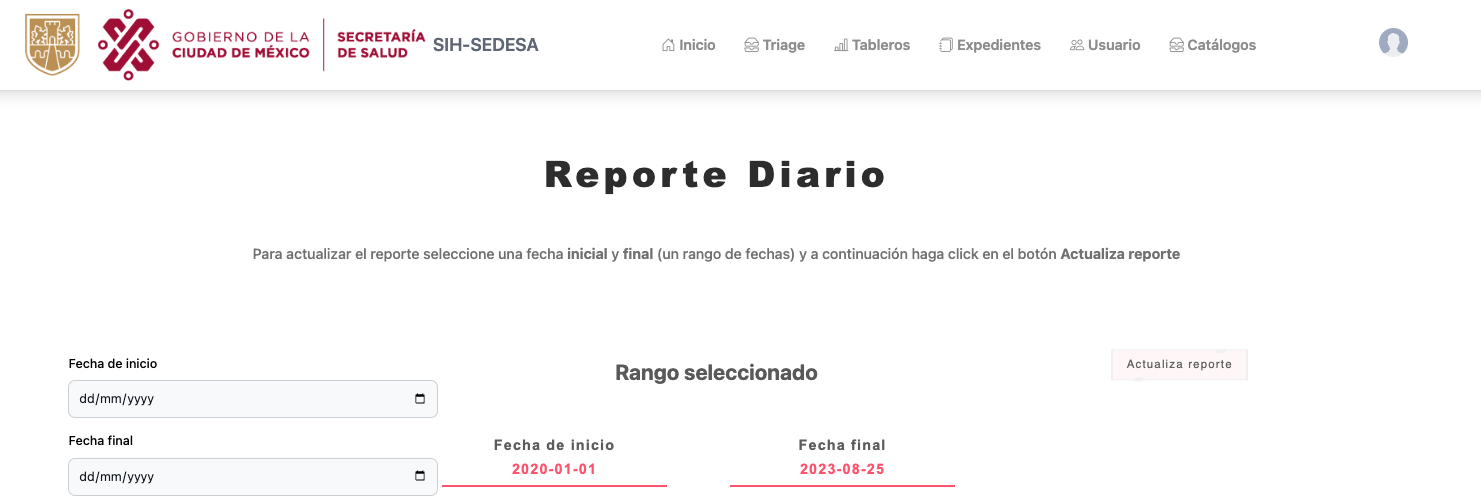
\includegraphics[width=\textwidth]{images/uso1.png}
    \caption{Menú superior de la aplicación SI-SEDESA}
    \label{fig:calendario_menu}
\end{figure}

Se observa que se tiene una sección para poder seleccionar y cambiar el rango de fechas deseado, al igual que se muestran textos que reflejan tanto la \textit{fecha de inicio} como la \textit{fecha final}.

La manera en que se actualiza el rango fechas es la siguiente:

\begin{enumerate}
    \item En el lado izquierdo, se encuentran dos botones los cuales al darle \textit{click} sobre ellos, se desplegará un calendario que permitirá al usuario seleccionar la fecha deseada como se observa en la Figura \ref{fig:calendario_desplegable}.

    \begin{figure}[ht!]
        \centering
        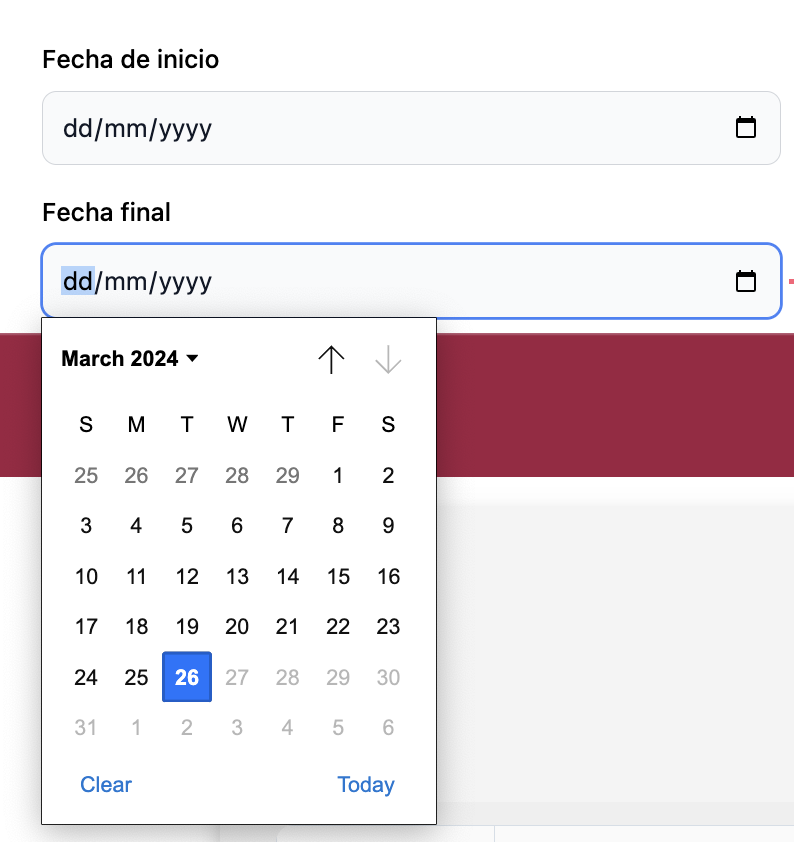
\includegraphics[width=0.3\textwidth]{images/uso3.png}
        \caption{Calendario que se despliega para que el usuario seleccione una nueva fecha de inicio o de fin.}
        \label{fig:calendario_desplegable}
    \end{figure}

    \item Una vez seleccionadas ambas fechas, se deberá hacer \textit{click} en el botón \textbf{Actualizar reporte} para poder aplicar los cambios dado el nuevo rango de fechas especificado y que se aplique una actualización a cada uno de los componentes.
\end{enumerate}


\section{Componentes finales del tablero de datos}

A continuación se mostrará como se ve el tablero de datos implementado por cada una de las páginas que lo conforman. 
\newpage

\begin{enumerate}
    \item \textbf{Componentes Página 1}

    Para la tabla que se encuentra en esta página se está usando una barra que permite al usuario desplazarse a lo largo de la tabla ya que al tener un número considerable de columnas se expande a lo largo de toda la página lo que anteriormente no era del  favorable. En la Figura \ref{fig:pag1_final_1} y en la Figura \ref{fig:pag1_final_2} se muestra el aspecto final de los componentes correspondientes a la primera página del tablero de datos.
    
    \begin{figure}[h!]
        \centering
        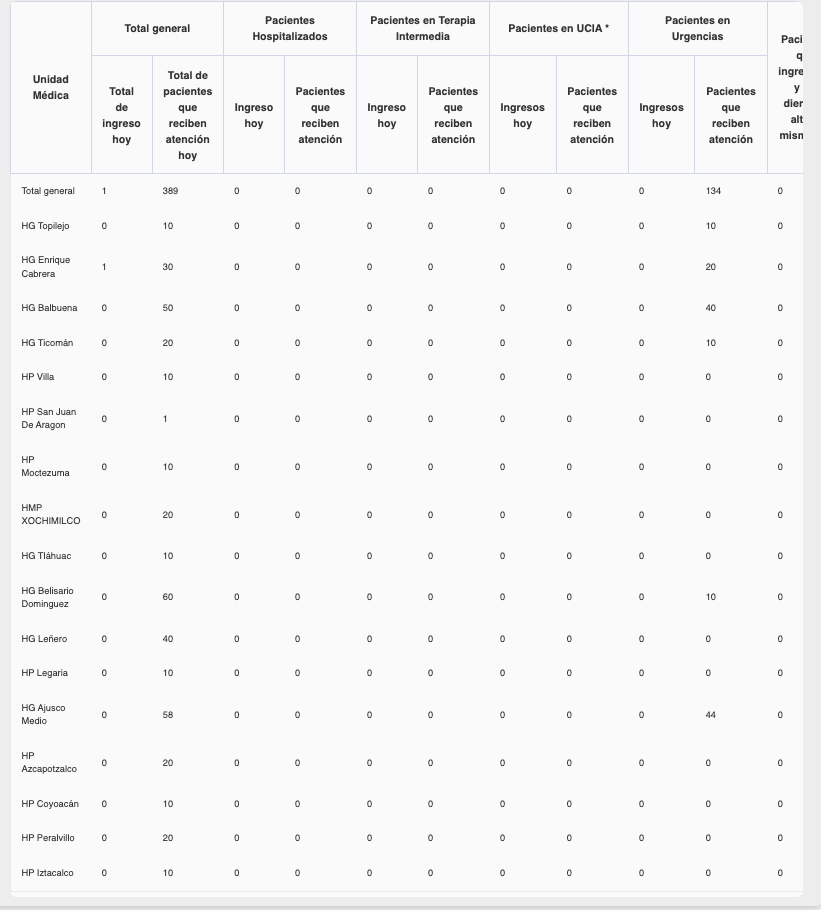
\includegraphics[width=0.75\textwidth]{images/pag1_tabla.png}
        \caption{Tabla correspondiente a la página 1 del tablero de datos.}
        \label{fig:pag1_final_1}
    \end{figure}

    \begin{figure}[h!]
        \centering
        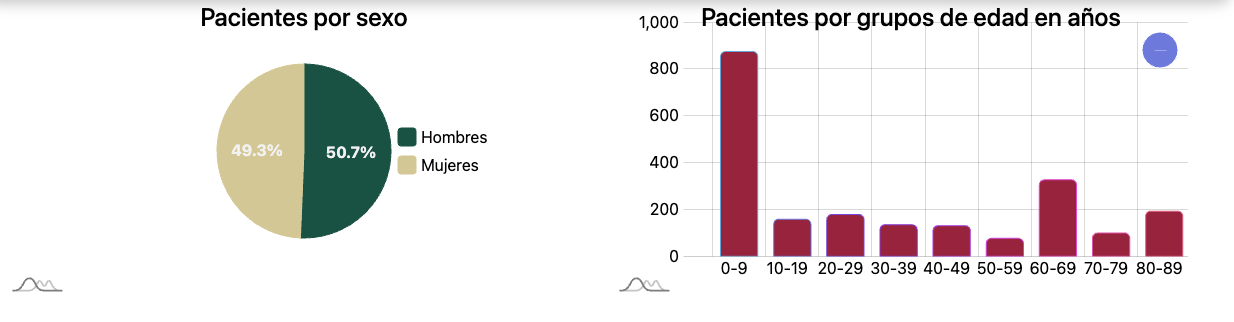
\includegraphics[width=0.8\textwidth]{images/pag1_graficas.png}
        \caption{Gráficas correspondientes a la página 1 del tablero de datos.}
        \label{fig:pag1_final_2}
    \end{figure}

    \newpage 
    \item \textbf{Componentes Página 2}

    De la misma manera en que la tabla contenida en la página 1, la tabla correspondiente a la página 2 también posee una barra desplazable. En la Figura \ref{fig:pag2_final_1} y en la Figura \ref{fig:pag2_final_2} se muestra el aspecto final de los componentes correspondientes a la segunda página del tablero de datos.

    \begin{figure}[h!]
        \centering
        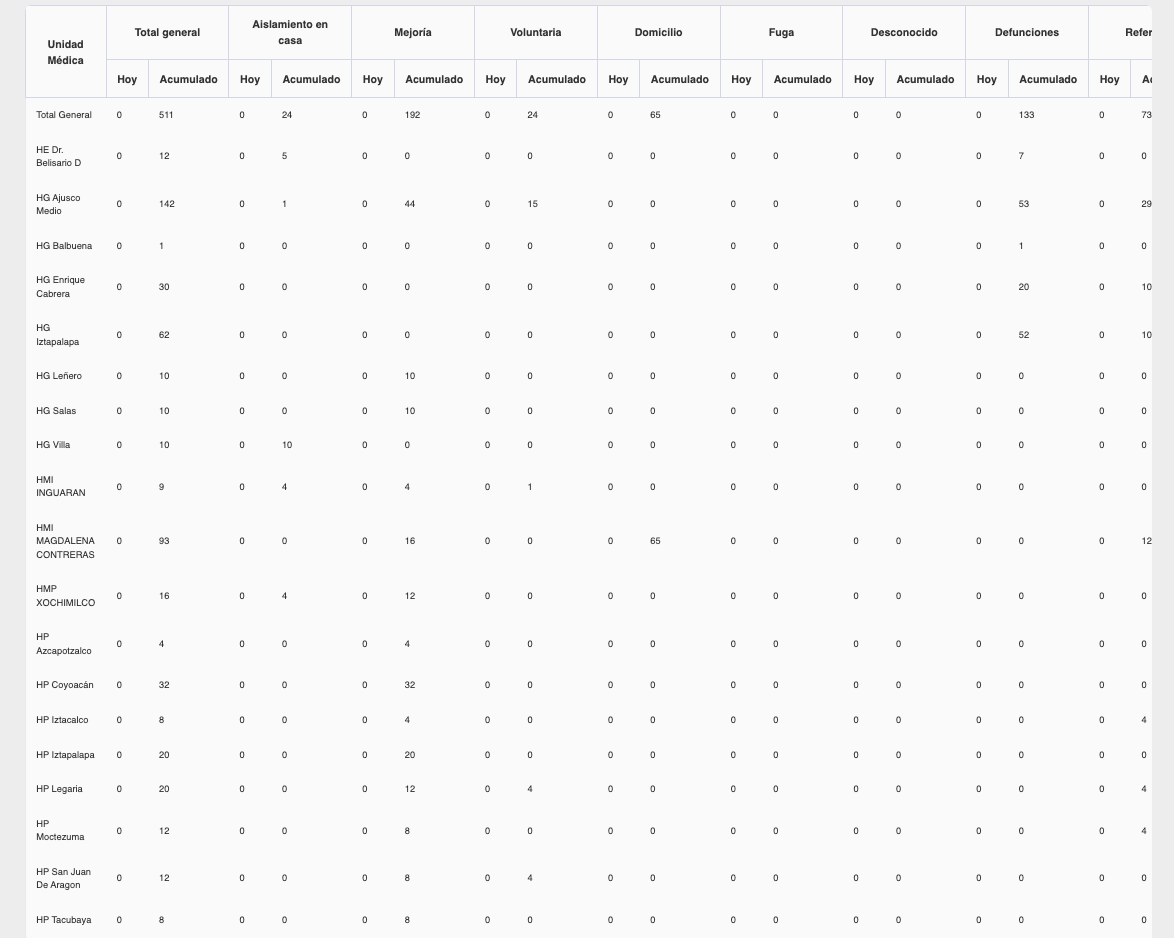
\includegraphics[width=0.9\textwidth]{images/pag2_tabla.png}
        \caption{Tabla correspondiente a la página 2 del tablero de datos.}
        \label{fig:pag2_final_1}
    \end{figure}

    \begin{figure}[h!]
        \centering
        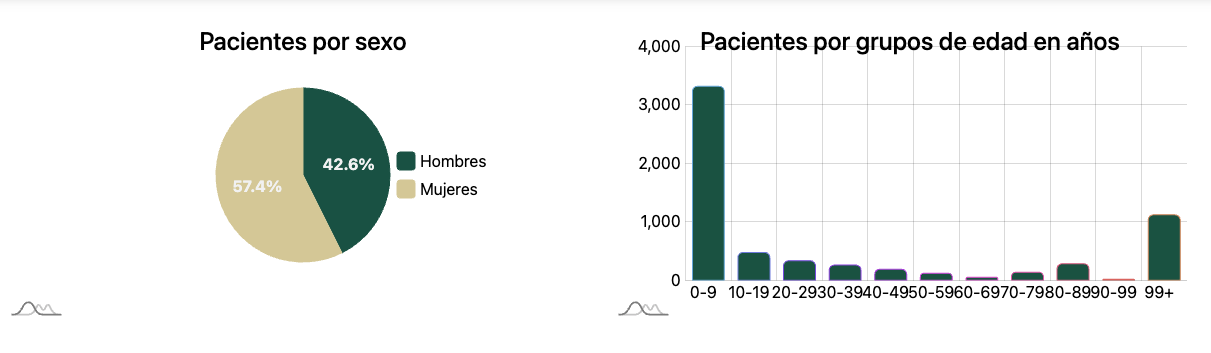
\includegraphics[width=0.9\textwidth]{images/pag2_graficas.png}
        \caption{Gráficas correspondientes a la página 2 del tablero de datos.}
        \label{fig:pag2_final_2}
    \end{figure}

    \newpage

    \item \textbf{Componentes Página 3}

    En lo que respecta  a la página 3, ambas gráficas muestran de manera correcta la información proporcionada, mientras que la tabla se sobre lapa sobre la gráfica de barras, esto está en proceso de corrección ya que hay una cantidad considerable de renglones que provoca este sobrelape. En la Figura \ref{fig:pag3_final} se muestra el aspecto final de los componentes correspondientes a la primera página del tablero de datos.
    
    \begin{figure}[h!]
        \centering
        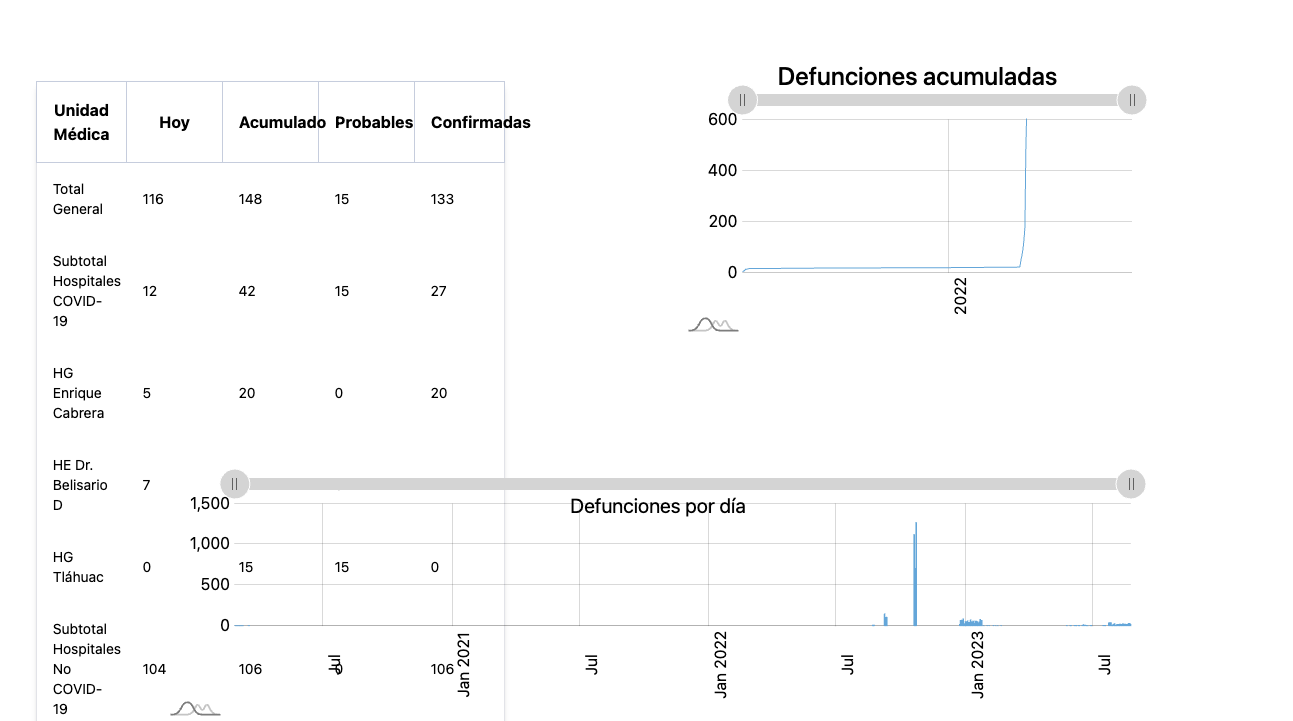
\includegraphics[width=0.8\textwidth]{images/pag3.png}
        \caption{Gráficas y tabla correspondientes a la página 3 del tablero de datos.}
        \label{fig:pag3_final}
    \end{figure}

    \item \textbf{Componentes Página 4}

    En esta página no ha habido ningún problema con la apariencia de las gráficas, únicamente hace falta un mayor volumen de datos para que se pueda apreciar de una manera más estética. En la Figura \ref{fig:pag4_final} se muestra el aspecto final de los componentes correspondientes a la primera página del tablero de datos.

    \begin{figure}[h!]
        \centering
        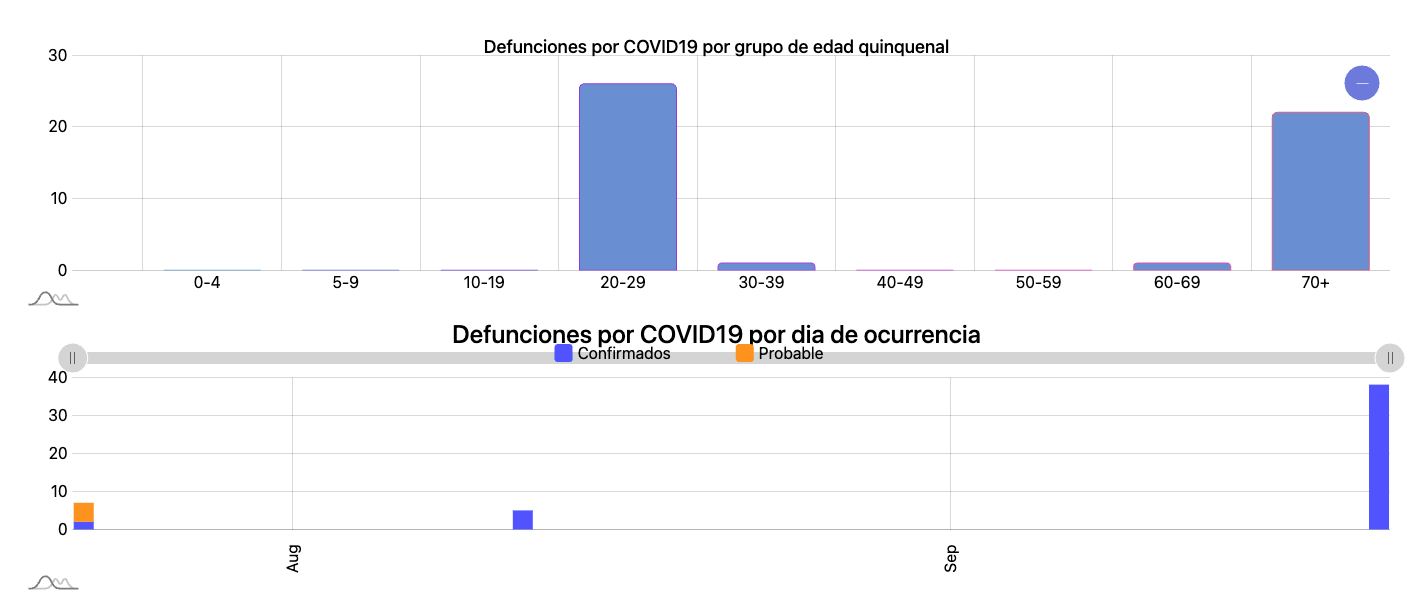
\includegraphics[width=0.8\textwidth]{images/pag4.png}
        \caption{Gráficas correspondientes a la página 4 del tablero de datos.}
        \label{fig:pag4_final}
    \end{figure}

    \newpage
    
    \item \textbf{Componentes Página 5}

    Al igual que la página anterior, se necesita un volumen de datos mayor para que la gráfica de barras se vea similar a lo que se mostró en el mockup. En la Figura \ref{fig:pag5_final} se muestra el aspecto final de los componentes correspondientes a la primera página del tablero de datos.

    \begin{figure}[h!]
        \centering
        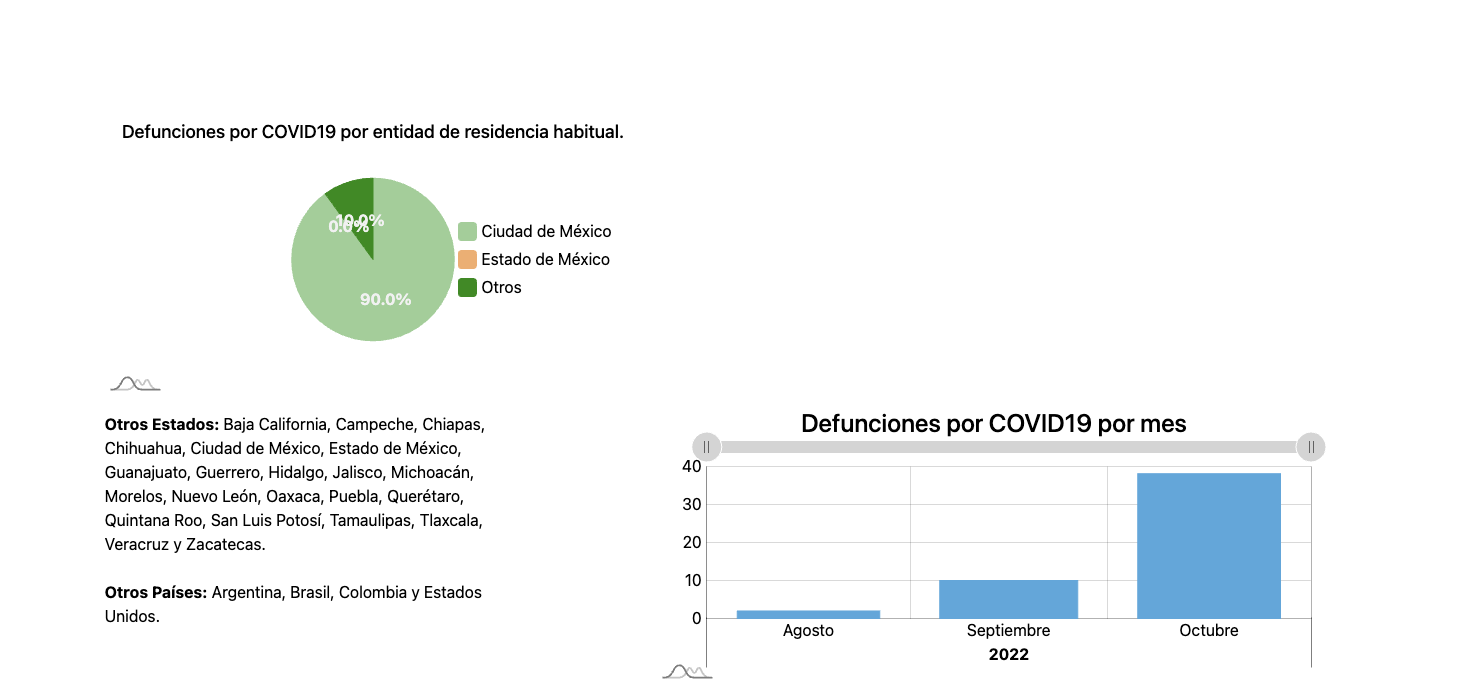
\includegraphics[width=0.75\textwidth]{images/pag5.png}
        \caption{Gráficas correspondientes a la página 5 del tablero de datos.}
        \label{fig:pag5_final}
    \end{figure}

    \item \textbf{Componentes Página 6}

    Por último en lo que respecta  la página 6, se presenta el mismo inconveniente de no contar con gran volumen de datos para que en la gráfica de barras que muestra el número de traslados por semana epidemiológica sea vea de mejor manera. En cuanto a la gráfica pastel que muestra los traslados por institución, la tabla \texttt{general.thospital} que es de dónde se obtiene la información de los hospitales aún no posee una columna que especifique a que institución pertenecen los hospitales, ya es algo que se solicitó a \textbf{SEDESA}, pero aún no se obtiene respuesta. Por lo que actualmente se están tomando en cuenta cada uno de los hospitales para la visualización de datos. En la Figura \ref{fig:pag5_final} se muestra el aspecto final de los componentes correspondientes a la primera página del tablero de datos.

    \begin{figure}[h!]
        \centering
        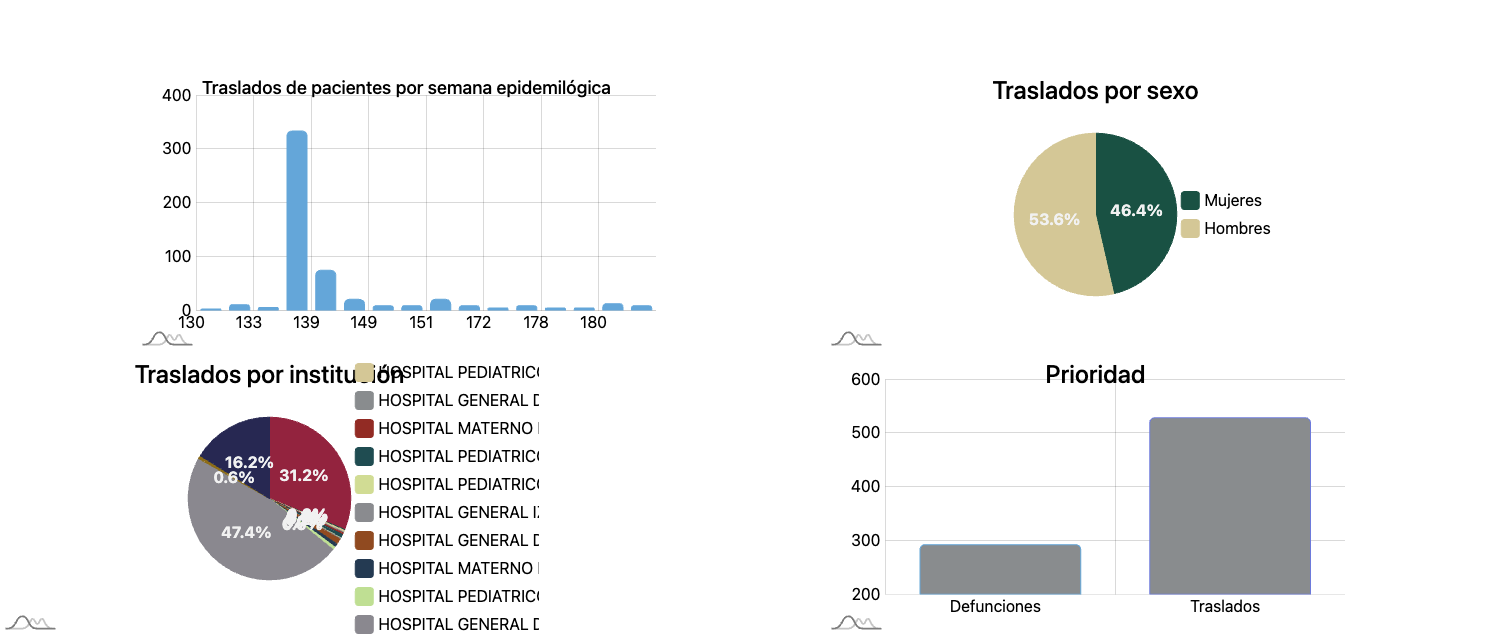
\includegraphics[width=0.85\textwidth]{images/pag6.png}
        \caption{Gráficas correspondientes a la página 6 del tablero de datos.}
        \label{fig:pag6_final}
    \end{figure}
    

    
    
\end{enumerate}




%-------------------------------------------------------------------
\section{Resumen}
En este capítulo se detalló la construcción final del tablero de datos que muestra información de los pacientes con COVID-19 internados en los hospitales pertenecientes a \textbf{SEDESA}, explicando su funcionamiento y la configuración de sus páginas. El tablero se compone de un calendario y un menú superior que permite la selección de diferentes secciones, incluyendo el "Reporte Diario", el cual carga inicialmente con parámetros de fechas predeterminados. Se describe el proceso para cambiar el rango de fechas y actualizar el reporte correspondiente.\\

Se presentan los componentes finales del tablero, mostrando las tablas y gráficas correspondientes a cada una de las seis páginas. Se destacan aspectos como la necesidad de barras desplazables para manejar grandes cantidades de datos dentro de las tablas, así como la mejora estética esperada con un mayor volumen de información. Se señalan algunos problemas pendientes de corrección, como el solapamiento de elementos en ciertas páginas y la falta de especificación de instituciones a las que pertenecen los hospitales.\\

El desarrollo del tablero se encuentra en proceso de optimización y ajustes, con la colaboración de \textbf{SEDESA} para garantizar su adecuada representación y funcionalidad.
